\documentclass[twoside]{book}

% Packages required by doxygen
\usepackage{fixltx2e}
\usepackage{calc}
\usepackage{doxygen}
\usepackage[export]{adjustbox} % also loads graphicx
\usepackage{graphicx}
\usepackage[utf8]{inputenc}
\usepackage{makeidx}
\usepackage{multicol}
\usepackage{multirow}
\PassOptionsToPackage{warn}{textcomp}
\usepackage{textcomp}
\usepackage[nointegrals]{wasysym}
\usepackage[table]{xcolor}

% Font selection
\usepackage[T1]{fontenc}
\usepackage[scaled=.90]{helvet}
\usepackage{courier}
\usepackage{amssymb}
\usepackage{sectsty}
\renewcommand{\familydefault}{\sfdefault}
\allsectionsfont{%
  \fontseries{bc}\selectfont%
  \color{darkgray}%
}
\renewcommand{\DoxyLabelFont}{%
  \fontseries{bc}\selectfont%
  \color{darkgray}%
}
\newcommand{\+}{\discretionary{\mbox{\scriptsize$\hookleftarrow$}}{}{}}

% Page & text layout
\usepackage{geometry}
\geometry{%
  a4paper,%
  top=2.5cm,%
  bottom=2.5cm,%
  left=2.5cm,%
  right=2.5cm%
}
\tolerance=750
\hfuzz=15pt
\hbadness=750
\setlength{\emergencystretch}{15pt}
\setlength{\parindent}{0cm}
\setlength{\parskip}{0.2cm}
\makeatletter
\renewcommand{\paragraph}{%
  \@startsection{paragraph}{4}{0ex}{-1.0ex}{1.0ex}{%
    \normalfont\normalsize\bfseries\SS@parafont%
  }%
}
\renewcommand{\subparagraph}{%
  \@startsection{subparagraph}{5}{0ex}{-1.0ex}{1.0ex}{%
    \normalfont\normalsize\bfseries\SS@subparafont%
  }%
}
\makeatother

% Headers & footers
\usepackage{fancyhdr}
\pagestyle{fancyplain}
\fancyhead[LE]{\fancyplain{}{\bfseries\thepage}}
\fancyhead[CE]{\fancyplain{}{}}
\fancyhead[RE]{\fancyplain{}{\bfseries\leftmark}}
\fancyhead[LO]{\fancyplain{}{\bfseries\rightmark}}
\fancyhead[CO]{\fancyplain{}{}}
\fancyhead[RO]{\fancyplain{}{\bfseries\thepage}}
\fancyfoot[LE]{\fancyplain{}{}}
\fancyfoot[CE]{\fancyplain{}{}}
\fancyfoot[RE]{\fancyplain{}{\bfseries\scriptsize Generated by Doxygen }}
\fancyfoot[LO]{\fancyplain{}{\bfseries\scriptsize Generated by Doxygen }}
\fancyfoot[CO]{\fancyplain{}{}}
\fancyfoot[RO]{\fancyplain{}{}}
\renewcommand{\footrulewidth}{0.4pt}
\renewcommand{\chaptermark}[1]{%
  \markboth{#1}{}%
}
\renewcommand{\sectionmark}[1]{%
  \markright{\thesection\ #1}%
}

% Indices & bibliography
\usepackage{natbib}
\usepackage[titles]{tocloft}
\setcounter{tocdepth}{3}
\setcounter{secnumdepth}{5}
\makeindex

% Hyperlinks (required, but should be loaded last)
\usepackage{ifpdf}
\ifpdf
  \usepackage[pdftex,pagebackref=true]{hyperref}
\else
  \usepackage[ps2pdf,pagebackref=true]{hyperref}
\fi
\hypersetup{%
  colorlinks=true,%
  linkcolor=blue,%
  citecolor=blue,%
  unicode%
}

% Custom commands
\newcommand{\clearemptydoublepage}{%
  \newpage{\pagestyle{empty}\cleardoublepage}%
}


%===== C O N T E N T S =====

\begin{document}

% Titlepage & ToC
\hypersetup{pageanchor=false,
             bookmarks=true,
             bookmarksnumbered=true,
             pdfencoding=unicode
            }
\pagenumbering{roman}
\begin{titlepage}
\vspace*{7cm}
\begin{center}%
{\Large Semester 2 Assignment \\[1ex]\large 1 }\\
\vspace*{1cm}
{\large Generated by Doxygen 1.8.10}\\
\end{center}
\end{titlepage}
\clearemptydoublepage
\tableofcontents
\clearemptydoublepage
\pagenumbering{arabic}
\hypersetup{pageanchor=true}

%--- Begin generated contents ---
\chapter{Hierarchical Index}
\section{Class Hierarchy}
This inheritance list is sorted roughly, but not completely, alphabetically\+:\begin{DoxyCompactList}
\item \contentsline{section}{Game\+Asset}{\pageref{classGameAsset}}{}
\begin{DoxyCompactList}
\item \contentsline{section}{Cube\+Asset}{\pageref{classCubeAsset}}{}
\end{DoxyCompactList}
\item \contentsline{section}{Game\+Asset\+Manager}{\pageref{classGameAssetManager}}{}
\item \contentsline{section}{Game\+World}{\pageref{classGameWorld}}{}
\item \contentsline{section}{S\+D\+L\+Window\+Deleter}{\pageref{structSDLWindowDeleter}}{}
\end{DoxyCompactList}

\chapter{Class Index}
\section{Class List}
Here are the classes, structs, unions and interfaces with brief descriptions\+:\begin{DoxyCompactList}
\item\contentsline{section}{\hyperlink{classCubeAsset}{Cube\+Asset} }{\pageref{classCubeAsset}}{}
\item\contentsline{section}{\hyperlink{classGameAsset}{Game\+Asset} }{\pageref{classGameAsset}}{}
\item\contentsline{section}{\hyperlink{classGameAssetManager}{Game\+Asset\+Manager} }{\pageref{classGameAssetManager}}{}
\item\contentsline{section}{\hyperlink{classGameWorld}{Game\+World} }{\pageref{classGameWorld}}{}
\item\contentsline{section}{\hyperlink{structSDLWindowDeleter}{S\+D\+L\+Window\+Deleter} }{\pageref{structSDLWindowDeleter}}{}
\end{DoxyCompactList}

\chapter{Class Documentation}
\hypertarget{classCubeAsset}{}\section{Cube\+Asset Class Reference}
\label{classCubeAsset}\index{Cube\+Asset@{Cube\+Asset}}
Inheritance diagram for Cube\+Asset\+:\begin{figure}[H]
\begin{center}
\leavevmode
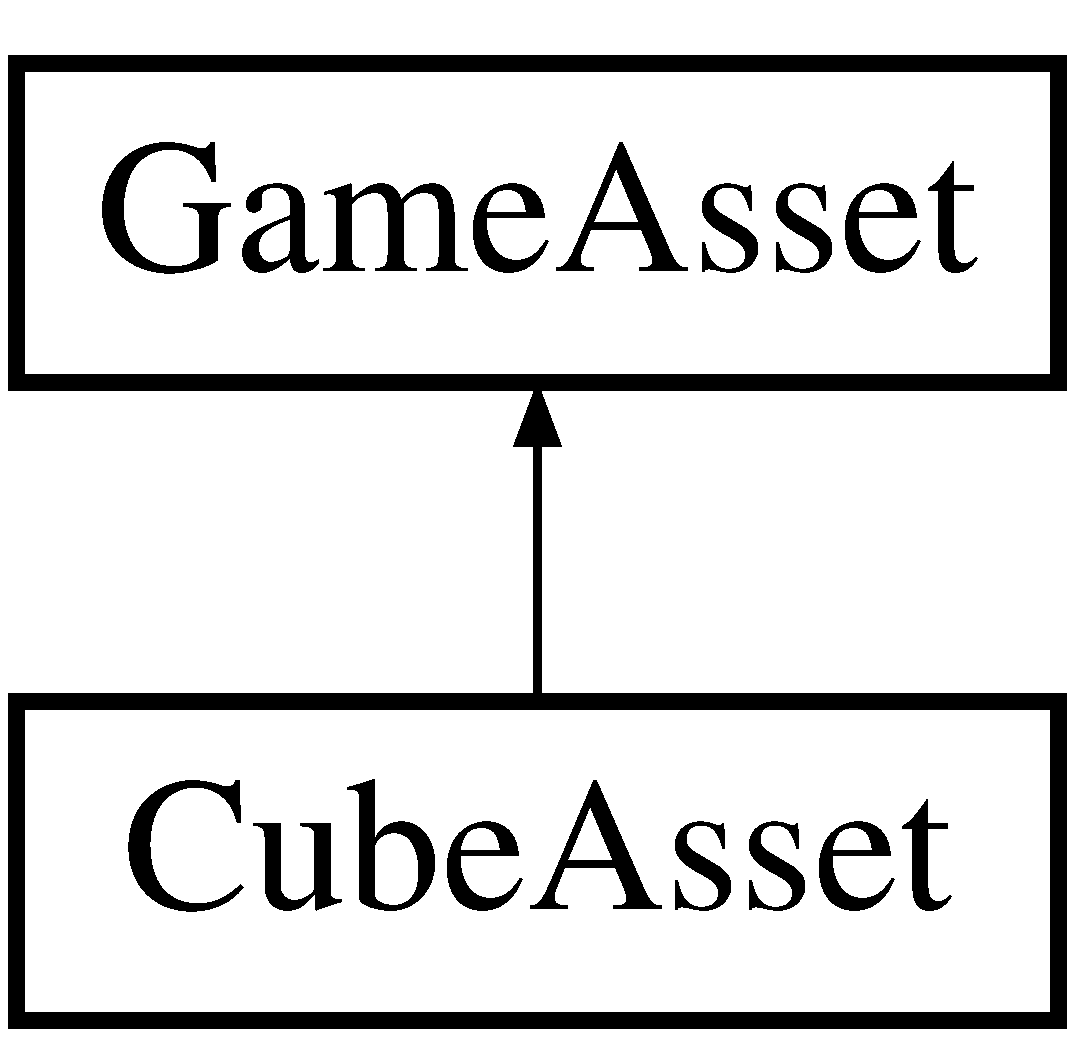
\includegraphics[height=2.000000cm]{classCubeAsset}
\end{center}
\end{figure}
\subsection*{Public Member Functions}
\begin{DoxyCompactItemize}
\item 
\hypertarget{classCubeAsset_a0252e564114a3cda7e3911ef95742a34}{}{\bfseries Cube\+Asset} (G\+Lfloat x, G\+Lfloat y, G\+Lfloat z)\label{classCubeAsset_a0252e564114a3cda7e3911ef95742a34}

\item 
\hypertarget{classCubeAsset_a1af568486056e254ffcf98fd99947bfe}{}virtual void {\bfseries Draw} (G\+Luint)\label{classCubeAsset_a1af568486056e254ffcf98fd99947bfe}

\end{DoxyCompactItemize}


The documentation for this class was generated from the following files\+:\begin{DoxyCompactItemize}
\item 
Cube\+Asset.\+h\item 
Cube\+Asset.\+cc\end{DoxyCompactItemize}

\hypertarget{classGameAsset}{}\section{Game\+Asset Class Reference}
\label{classGameAsset}\index{Game\+Asset@{Game\+Asset}}
Inheritance diagram for Game\+Asset\+:\begin{figure}[H]
\begin{center}
\leavevmode
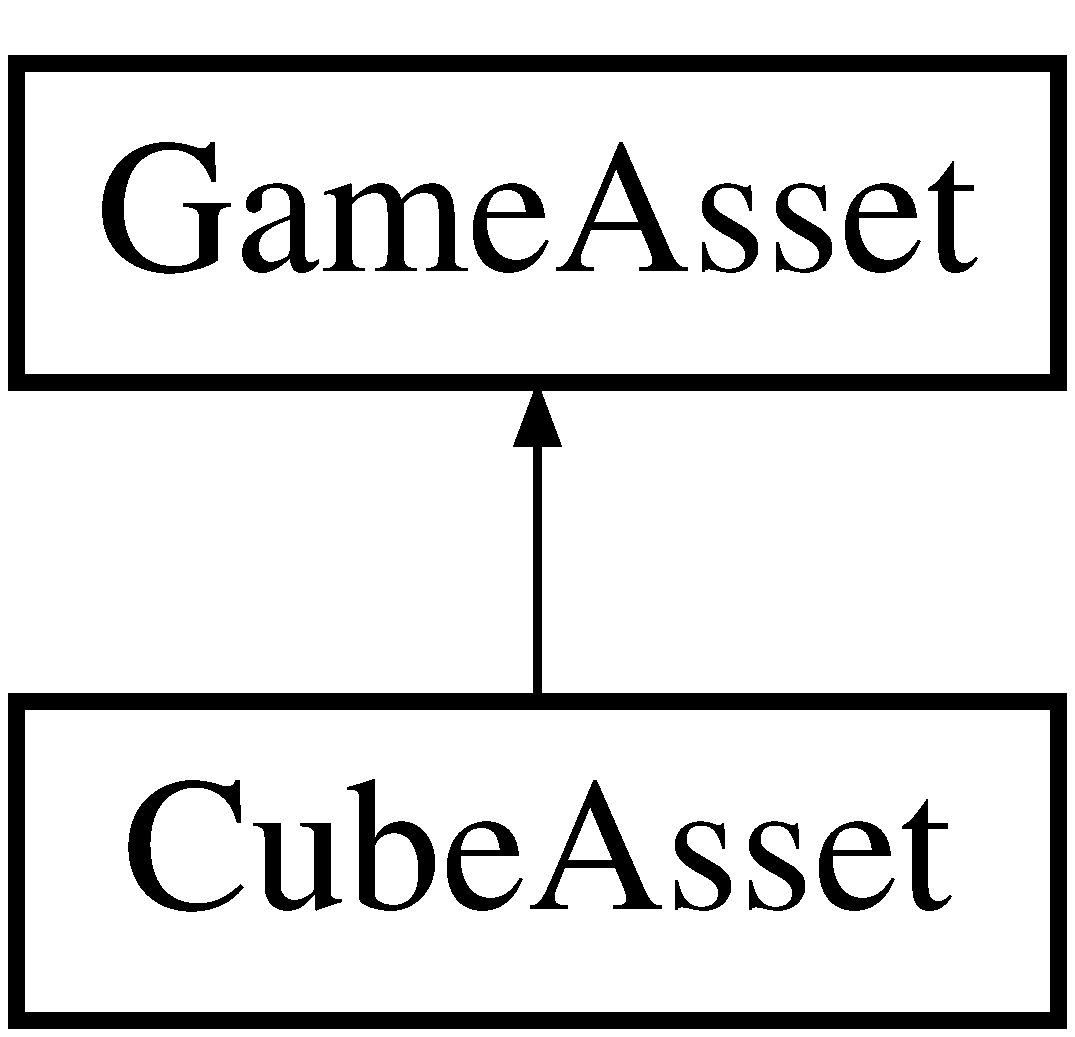
\includegraphics[height=2.000000cm]{classGameAsset}
\end{center}
\end{figure}
\subsection*{Public Member Functions}
\begin{DoxyCompactItemize}
\item 
\hypertarget{classGameAsset_a961aa51ca0a9961fc584c0b5d5431300}{}virtual void {\bfseries Draw} (G\+Luint)=0\label{classGameAsset_a961aa51ca0a9961fc584c0b5d5431300}

\end{DoxyCompactItemize}


The documentation for this class was generated from the following file\+:\begin{DoxyCompactItemize}
\item 
Game\+Asset.\+h\end{DoxyCompactItemize}

\hypertarget{classGameAssetManager}{}\section{Game\+Asset\+Manager Class Reference}
\label{classGameAssetManager}\index{Game\+Asset\+Manager@{Game\+Asset\+Manager}}


{\ttfamily \#include $<$Game\+Asset\+Manager.\+h$>$}

\subsection*{Public Member Functions}
\begin{DoxyCompactItemize}
\item 
\hyperlink{classGameAssetManager_aaa0d58e276cc10ad91a7457085598a71}{Game\+Asset\+Manager} (Application\+Mode)
\item 
virtual \hyperlink{classGameAssetManager_a1270bd61ecbcca563f079803e40c9b77}{$\sim$\+Game\+Asset\+Manager} ()
\item 
\hyperlink{classGameAssetManager_a2c9adcb72faa154c87eadc9bafe5269d}{Game\+Asset\+Manager} (\hyperlink{classGameAssetManager}{Game\+Asset\+Manager} const \&)
\item 
\hyperlink{classGameAssetManager_a44f6e2fd6b8ff1dd64e5697f1be7386d}{Game\+Asset\+Manager} (\hyperlink{classGameAssetManager}{Game\+Asset\+Manager} const \&\&)
\item 
void \hyperlink{classGameAssetManager_ac72678a4ad5378c685aa6bae84a4e712}{operator=} (\hyperlink{classGameAssetManager}{Game\+Asset\+Manager} const \&)
\item 
void \hyperlink{classGameAssetManager_ad3de8ff00d55ba04728b1de8213b2349}{Add\+Asset} (std\+::shared\+\_\+ptr$<$ \hyperlink{classGameAsset}{Game\+Asset} $>$)
\item 
void \hyperlink{classGameAssetManager_a32837132bd70a9a9ed537323c2d3d886}{Draw} ()
\end{DoxyCompactItemize}


\subsection{Detailed Description}
\hyperlink{classGameAssetManager}{Game\+Asset\+Manager} is a container for Game\+Assets. It also provides utility functions to to create a simple Open\+G\+L program that can be used to draw a simple \hyperlink{classGameAsset}{Game\+Asset}. 

\subsection{Constructor \& Destructor Documentation}
\hypertarget{classGameAssetManager_aaa0d58e276cc10ad91a7457085598a71}{}\index{Game\+Asset\+Manager@{Game\+Asset\+Manager}!Game\+Asset\+Manager@{Game\+Asset\+Manager}}
\index{Game\+Asset\+Manager@{Game\+Asset\+Manager}!Game\+Asset\+Manager@{Game\+Asset\+Manager}}
\subsubsection[{Game\+Asset\+Manager(\+Application\+Mode)}]{\setlength{\rightskip}{0pt plus 5cm}Game\+Asset\+Manager\+::\+Game\+Asset\+Manager (
\begin{DoxyParamCaption}
\item[{Application\+Mode}]{mode}
\end{DoxyParamCaption}
)\hspace{0.3cm}{\ttfamily [explicit]}}\label{classGameAssetManager_aaa0d58e276cc10ad91a7457085598a71}
Creates a \hyperlink{classGameAssetManager}{Game\+Asset\+Manager} to load the correct shaders based on the Application\+Mode. \hypertarget{classGameAssetManager_a1270bd61ecbcca563f079803e40c9b77}{}\index{Game\+Asset\+Manager@{Game\+Asset\+Manager}!````~Game\+Asset\+Manager@{$\sim$\+Game\+Asset\+Manager}}
\index{````~Game\+Asset\+Manager@{$\sim$\+Game\+Asset\+Manager}!Game\+Asset\+Manager@{Game\+Asset\+Manager}}
\subsubsection[{$\sim$\+Game\+Asset\+Manager()}]{\setlength{\rightskip}{0pt plus 5cm}Game\+Asset\+Manager\+::$\sim$\+Game\+Asset\+Manager (
\begin{DoxyParamCaption}
{}
\end{DoxyParamCaption}
)\hspace{0.3cm}{\ttfamily [virtual]}}\label{classGameAssetManager_a1270bd61ecbcca563f079803e40c9b77}
Deletes a \hyperlink{classGameAssetManager}{Game\+Asset\+Manager}, in particular it will clean up any modifications to the Open\+G\+L state. \hypertarget{classGameAssetManager_a2c9adcb72faa154c87eadc9bafe5269d}{}\index{Game\+Asset\+Manager@{Game\+Asset\+Manager}!Game\+Asset\+Manager@{Game\+Asset\+Manager}}
\index{Game\+Asset\+Manager@{Game\+Asset\+Manager}!Game\+Asset\+Manager@{Game\+Asset\+Manager}}
\subsubsection[{Game\+Asset\+Manager(\+Game\+Asset\+Manager const \&)}]{\setlength{\rightskip}{0pt plus 5cm}Game\+Asset\+Manager\+::\+Game\+Asset\+Manager (
\begin{DoxyParamCaption}
\item[{{\bf Game\+Asset\+Manager} const \&}]{the\+\_\+manager}
\end{DoxyParamCaption}
)}\label{classGameAssetManager_a2c9adcb72faa154c87eadc9bafe5269d}
Unimplemented copy constructor -- this means that the \hyperlink{classGameAssetManager}{Game\+Asset\+Manager} may not work as you\textquotesingle{}d expect when being copied. \hypertarget{classGameAssetManager_a44f6e2fd6b8ff1dd64e5697f1be7386d}{}\index{Game\+Asset\+Manager@{Game\+Asset\+Manager}!Game\+Asset\+Manager@{Game\+Asset\+Manager}}
\index{Game\+Asset\+Manager@{Game\+Asset\+Manager}!Game\+Asset\+Manager@{Game\+Asset\+Manager}}
\subsubsection[{Game\+Asset\+Manager(\+Game\+Asset\+Manager const \&\&)}]{\setlength{\rightskip}{0pt plus 5cm}Game\+Asset\+Manager\+::\+Game\+Asset\+Manager (
\begin{DoxyParamCaption}
\item[{{\bf Game\+Asset\+Manager} const \&\&}]{the\+\_\+manager}
\end{DoxyParamCaption}
)}\label{classGameAssetManager_a44f6e2fd6b8ff1dd64e5697f1be7386d}
Unimplemented move constructor -- this unimplemented method violates the C++11 move semantics for \hyperlink{classGameAssetManager}{Game\+Asset\+Manager}. 

\subsection{Member Function Documentation}
\hypertarget{classGameAssetManager_ad3de8ff00d55ba04728b1de8213b2349}{}\index{Game\+Asset\+Manager@{Game\+Asset\+Manager}!Add\+Asset@{Add\+Asset}}
\index{Add\+Asset@{Add\+Asset}!Game\+Asset\+Manager@{Game\+Asset\+Manager}}
\subsubsection[{Add\+Asset(std\+::shared\+\_\+ptr$<$ Game\+Asset $>$)}]{\setlength{\rightskip}{0pt plus 5cm}void Game\+Asset\+Manager\+::\+Add\+Asset (
\begin{DoxyParamCaption}
\item[{std\+::shared\+\_\+ptr$<$ {\bf Game\+Asset} $>$}]{the\+\_\+asset}
\end{DoxyParamCaption}
)}\label{classGameAssetManager_ad3de8ff00d55ba04728b1de8213b2349}
Adds a \hyperlink{classGameAsset}{Game\+Asset} to the scene graph. \hypertarget{classGameAssetManager_a32837132bd70a9a9ed537323c2d3d886}{}\index{Game\+Asset\+Manager@{Game\+Asset\+Manager}!Draw@{Draw}}
\index{Draw@{Draw}!Game\+Asset\+Manager@{Game\+Asset\+Manager}}
\subsubsection[{Draw()}]{\setlength{\rightskip}{0pt plus 5cm}void Game\+Asset\+Manager\+::\+Draw (
\begin{DoxyParamCaption}
{}
\end{DoxyParamCaption}
)}\label{classGameAssetManager_a32837132bd70a9a9ed537323c2d3d886}
Draws each \hyperlink{classGameAsset}{Game\+Asset} in the scene graph. \hypertarget{classGameAssetManager_ac72678a4ad5378c685aa6bae84a4e712}{}\index{Game\+Asset\+Manager@{Game\+Asset\+Manager}!operator=@{operator=}}
\index{operator=@{operator=}!Game\+Asset\+Manager@{Game\+Asset\+Manager}}
\subsubsection[{operator=(\+Game\+Asset\+Manager const \&)}]{\setlength{\rightskip}{0pt plus 5cm}void Game\+Asset\+Manager\+::operator= (
\begin{DoxyParamCaption}
\item[{{\bf Game\+Asset\+Manager} const \&}]{the\+\_\+manager}
\end{DoxyParamCaption}
)}\label{classGameAssetManager_ac72678a4ad5378c685aa6bae84a4e712}
Unimplemented assisgnment operator -- violates the expected semantics for assignment in C++11. 

The documentation for this class was generated from the following files\+:\begin{DoxyCompactItemize}
\item 
Game\+Asset\+Manager.\+h\item 
Game\+Asset\+Manager.\+cc\end{DoxyCompactItemize}

\hypertarget{classGameWorld}{}\section{Game\+World Class Reference}
\label{classGameWorld}\index{Game\+World@{Game\+World}}


{\ttfamily \#include $<$Game\+World.\+h$>$}

\subsection*{Public Member Functions}
\begin{DoxyCompactItemize}
\item 
\hyperlink{classGameWorld_a17a84e57a80600961088afc753036f89}{Game\+World} (Application\+Mode)
\item 
void \hyperlink{classGameWorld_a275418607d8286979b276f165ad5876b}{Draw} ()
\end{DoxyCompactItemize}


\subsection{Detailed Description}
\hyperlink{classGameWorld}{Game\+World} allows us to separate the management of the game world from the nuts and bolts of game loop initialisation. The \hyperlink{classGameWorld}{Game\+World} currently has a very simplified scene graph consisiting of a single \hyperlink{classGameAssetManager}{Game\+Asset\+Manager}. 

\subsection{Constructor \& Destructor Documentation}
\hypertarget{classGameWorld_a17a84e57a80600961088afc753036f89}{}\index{Game\+World@{Game\+World}!Game\+World@{Game\+World}}
\index{Game\+World@{Game\+World}!Game\+World@{Game\+World}}
\subsubsection[{Game\+World(\+Application\+Mode)}]{\setlength{\rightskip}{0pt plus 5cm}Game\+World\+::\+Game\+World (
\begin{DoxyParamCaption}
\item[{Application\+Mode}]{mode}
\end{DoxyParamCaption}
)}\label{classGameWorld_a17a84e57a80600961088afc753036f89}
We thread the Application\+Mode through the \hyperlink{classGameWorld}{Game\+World} ss we want to read it in from the user. Threading the state through the various function calls is preferable (in this case) to having some kind of global state. 

\subsection{Member Function Documentation}
\hypertarget{classGameWorld_a275418607d8286979b276f165ad5876b}{}\index{Game\+World@{Game\+World}!Draw@{Draw}}
\index{Draw@{Draw}!Game\+World@{Game\+World}}
\subsubsection[{Draw()}]{\setlength{\rightskip}{0pt plus 5cm}void Game\+World\+::\+Draw (
\begin{DoxyParamCaption}
{}
\end{DoxyParamCaption}
)}\label{classGameWorld_a275418607d8286979b276f165ad5876b}
Calling \hyperlink{classGameWorld_a275418607d8286979b276f165ad5876b}{Draw()} will draw the entire world. 

The documentation for this class was generated from the following files\+:\begin{DoxyCompactItemize}
\item 
Game\+World.\+h\item 
Game\+World.\+cc\end{DoxyCompactItemize}

\hypertarget{structSDLWindowDeleter}{}\section{S\+D\+L\+Window\+Deleter Struct Reference}
\label{structSDLWindowDeleter}\index{S\+D\+L\+Window\+Deleter@{S\+D\+L\+Window\+Deleter}}
\subsection*{Public Member Functions}
\begin{DoxyCompactItemize}
\item 
\hypertarget{structSDLWindowDeleter_a2aedcc99c3756ae090c38badabeb10b1}{}void {\bfseries operator()} (S\+D\+L\+\_\+\+Window $\ast$window)\label{structSDLWindowDeleter_a2aedcc99c3756ae090c38badabeb10b1}

\end{DoxyCompactItemize}


The documentation for this struct was generated from the following file\+:\begin{DoxyCompactItemize}
\item 
main.\+cc\end{DoxyCompactItemize}

%--- End generated contents ---

% Index
\backmatter
\newpage
\phantomsection
\clearemptydoublepage
\addcontentsline{toc}{chapter}{Index}
\printindex

\end{document}
